\documentclass{article}
\usepackage{amsmath}
\usepackage{amssymb}
\usepackage{graphicx}
\usepackage{hyperref}
\usepackage[version=4]{mhchem}


\begin{document}
As shown in the figure below, in \(\triangle A B C, \angle C A B=2 \angle A B C\). \(C D\) is the angle bisector of \(\angle A C B\). Show that \(B C=A C+A D\).

Solution:
Method 1:\\
\centering
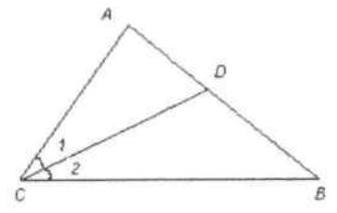
\includegraphics[width=\textwidth]{images/056.jpg}

Draw \(D E\) so that \(C E=A C\). Since \(\angle 1=\angle 2\), and \(C D=C D\), we have \(\triangle A C D \cong \triangle E C D\). Therefore \(\angle C E D=\angle C A B\), and \(A D=D E\).

Since \(\angle C A B=2 \angle A B C, \angle C E D=2 \angle A B C\), and \(\angle C E D=\)\\
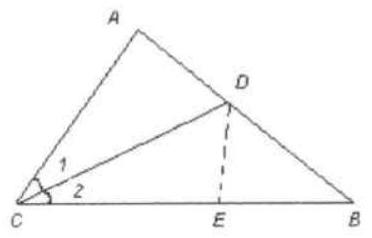
\includegraphics[width=\textwidth]{images/056(1).jpg} \(\angle D B E+\angle E D B\).

Hence \(\angle E D B=\angle E B D \Rightarrow D E=E B\).\\
Therefore \(B C=C E+E B=A C+D E=A C+A D\).\\
Method 2:\\
Extend \(C A\) to \(E\) such that \(A E=A D\). Therefore \(\angle E=\angle A D E\), and \(\angle C A B=2 \angle E\).\\
Since \(\angle C A B=2 \angle A B C, \angle E=\angle A B C\).\\
Since \(\angle 1=\angle 2\) and \(C D=C D, \triangle C E D \cong \triangle C B D\).\\
\centering
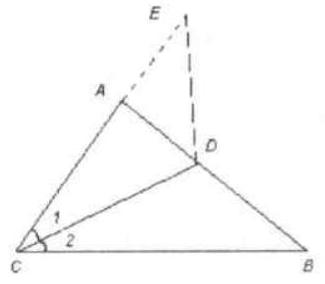
\includegraphics[width=\textwidth]{images/056(2).jpg}

Therefore \(C E=C B . B C=C E=C A+A E=C A+A D\).


Method 3:\\
Extend \(C A\) to \(E\) so that \(C E=C B\). Then \(\triangle C D E \cong \triangle C D B, \angle E\) \(=\angle B\).

Since \(\angle A=2 \angle B\), and \(\angle A=\angle E+\angle A D E\), so \(2 \angle B=\angle E\)\\
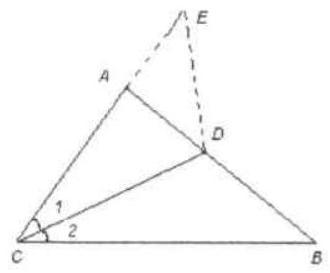
\includegraphics[width=\textwidth]{images/057.jpg} \(+\angle A D E\) or \(2 \angle E=\angle E+\angle A D E\), or \(\angle E=\angle A D E\), i.e, triangle \(A D E\) is an isosceles triangle with \(A D=A E\). Therefore \(B C=C A+A E=A C+A D\).


\end{document}
